\documentclass[tikz]{standalone}
\usepackage[compat=1.1.0]{tikz-feynman}

% feynman diagrams how-to

\begin{document}
\section{Problems}
\begin{itemize}
    \item how to change blob size?
\end{itemize}
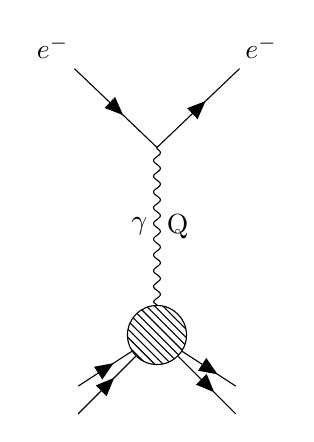
\begin{tikzpicture}
    \begin{feynman}
	\def\length{1 cm};
	% \vertex (ei1) {\(e^-\)};
	% \vertex[below right=\length and \length of ei1] (a);
	% \vertex[above right=\length and \length of a] (eo1) {\(e^-\)};
	% somehow thses statements will produce unequal length on left and right side, that's quite wired
	\vertex (a);
	\vertex[above left=\length and \length of a] (ei1) {\(e^-\)};
	\vertex[above right=\length and \length of a] (eo1) {\(e^-\)};
	\vertex[blob, below=2*\length of a] (b) {}; % blob must have content, even blank {}
	\vertex[below left=\length and \length of b] (pi1);
	\vertex[above=1em of pi1] (pi2);
	\vertex[below right=\length and \length of b] (po1);
	\vertex[above=1em of po1] (po2);

	\diagram*{
	    (ei1) -- [fermion] (a) -- [fermion] (eo1),
	    (a) -- [photon, edge label={Q}, edge label'=$\gamma$] (b),
	    (pi1) -- [fermion] (b),
	    (pi2) -- [fermion] (b),
	    (b) -- [fermion] (po1),
	    (b) -- [fermion] (po2),
	    };
    \end{feynman}
\end{tikzpicture}
\end{document}
